\experiment{IPC Using Shared Memory}{11/10/2023}

\section{Aim}
Implement programs for IPC using Shared Memory.

\section{Algorithm}
\subsection{Algorithm for Writing to Shared Memory}
\begin{enumerate}
   \item Start
   \item Generate a unique key using ftok() function
   \item Create a shared memory segment using shmget() function with key, size, and flags
   \item Attach the process to the shared memory segment using shmat() function
   \item Get the address of the shared memory segment and print it
   \item Prompt the user to enter data to write to shared memory
   \item Read the data entered by the user into a buffer
   \item Copy the data from the buffer to the shared memory using strcpy() function
   \item Print the data written to the shared memory
   \item Detach the process from the shared memory segment using shmdt() function
   \item Stop
\end{enumerate}

\subsection{Algorithm for Reading from Shared Memory}
\begin{enumerate}
   \item Start
   \item Generate a unique key using ftok() function
   \item Get the identifier of the existing shared memory segment using shmget() function with key, size, and flags
   \item Attach the process to the shared memory segment using shmat() function
   \item Get the address of the shared memory segment and print it
   \item Read the data from the shared memory into a buffer
   \item Print the data read from the shared memory
   \item Detach the process from the shared memory segment using shmdt() function
   \item Destroy the shared memory segment using shmctl() function with IPC\_RMID flag
   \item Stop
\end{enumerate}

\section{C Program - Write to shared memory}
\begin{lstlisting}[label={list:c_program:queue}]
#include <sys/ipc.h>
#include <sys/shm.h>
#include <stdio.h>
#include <string.h>

int main()
{
    key_t key = ftok("shmfile", 43); // Generate a unique key
    int shmid = shmget(key, 1024, 0666 | IPC_CREAT); // Create a shared memory segment

    printf("Identifier for shared memory is %d\n", shmid);

    void *shared_memory = shmat(shmid, NULL, 0); // Attach the process to the shared memory segment
    printf("Process attached at %p\n", shared_memory);

    printf("Enter data to write to shared memory: ");
    char buff[100];
    scanf("%s", buff);

    strcpy(shared_memory, buff); // Copy data from buffer to shared memory
    printf("Data written to shared memory is: %s\n", (char *)shared_memory);

    shmdt(shared_memory); // Detach from shared memory

    return 0;
}
\end{lstlisting}
\section{C Program - Read from shared memory}
\begin{lstlisting}[label={list:c_program:queue}]
#include <sys/ipc.h>
#include <sys/shm.h>
#include <stdio.h>
#include <string.h>

int main()
{
    key_t key = ftok("shmfile", 43); // Generate a unique key
    int shmid = shmget(key, 1024, 0666); // Get the identifier of the existing shared memory segment

    printf("Identifier for shared memory is: %d\n", shmid);

    void *shared_memory = shmat(shmid, NULL, 0); // Attach the process to the shared memory segment
    printf("Process attached at %p\n", shared_memory);

    char buff[100];
    printf("Data read from shared memory is: %s\n", (char *)shared_memory);

    shmdt(shared_memory); // Detach from shared memory
    shmctl(shmid, IPC_RMID, NULL); // Destroy shared memory

    return 0;
}
\end{lstlisting}
\section{Output}
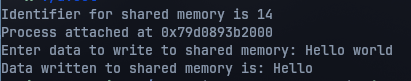
\includegraphics[]{Cycle_2//Outputs/writeShraed.png}\\
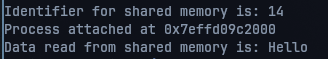
\includegraphics[]{Cycle_2//Outputs/readShared.png}


\section{Result}
Successfully implemented IPC using shared memory.